\section{EXPERIMENTAL RESULTS AND DISCUSSION}

The performance of the predictive models was evaluated using the Root Mean Squared Error (RMSE), the Mean Absolute Error (MAE), and the Coefficient of Determination ($R^2$). The $R^2$ score represents the proportion of the variance in the dependent variable that is predictable from the independent variables, whereas RMSE and MAE measure the average magnitude of the errors in kilograms of fuel.

The consolidated results of the models evaluated on the test set are presented in Table \ref{tab:models_summary}.

\begin{table}[htbp]
\caption{Comparison of Machine Learning Models}
\label{tab:models_summary}
\centering
\begin{tabular}{lccc}
\hline
\textbf{Model} & \textbf{RMSE} & \textbf{MAE} & \textbf{$R^2$} \\
\hline
Gradient Boosting & 35.19 & 22.71 & 0.5887 \\
XGBoost & 35.31 & 22.70 & 0.5858 \\
LightGBM & 35.34 & 22.72 & 0.5852 \\
Random Forest & 35.44 & 22.87 & 0.5829 \\
CatBoost & 36.07 & 23.28 & 0.5679 \\
Linear Regression & 38.23 & 24.60 & 0.5147 \\
\hline
\end{tabular}
\end{table}

\begin{figure}[htbp]
    \centering
    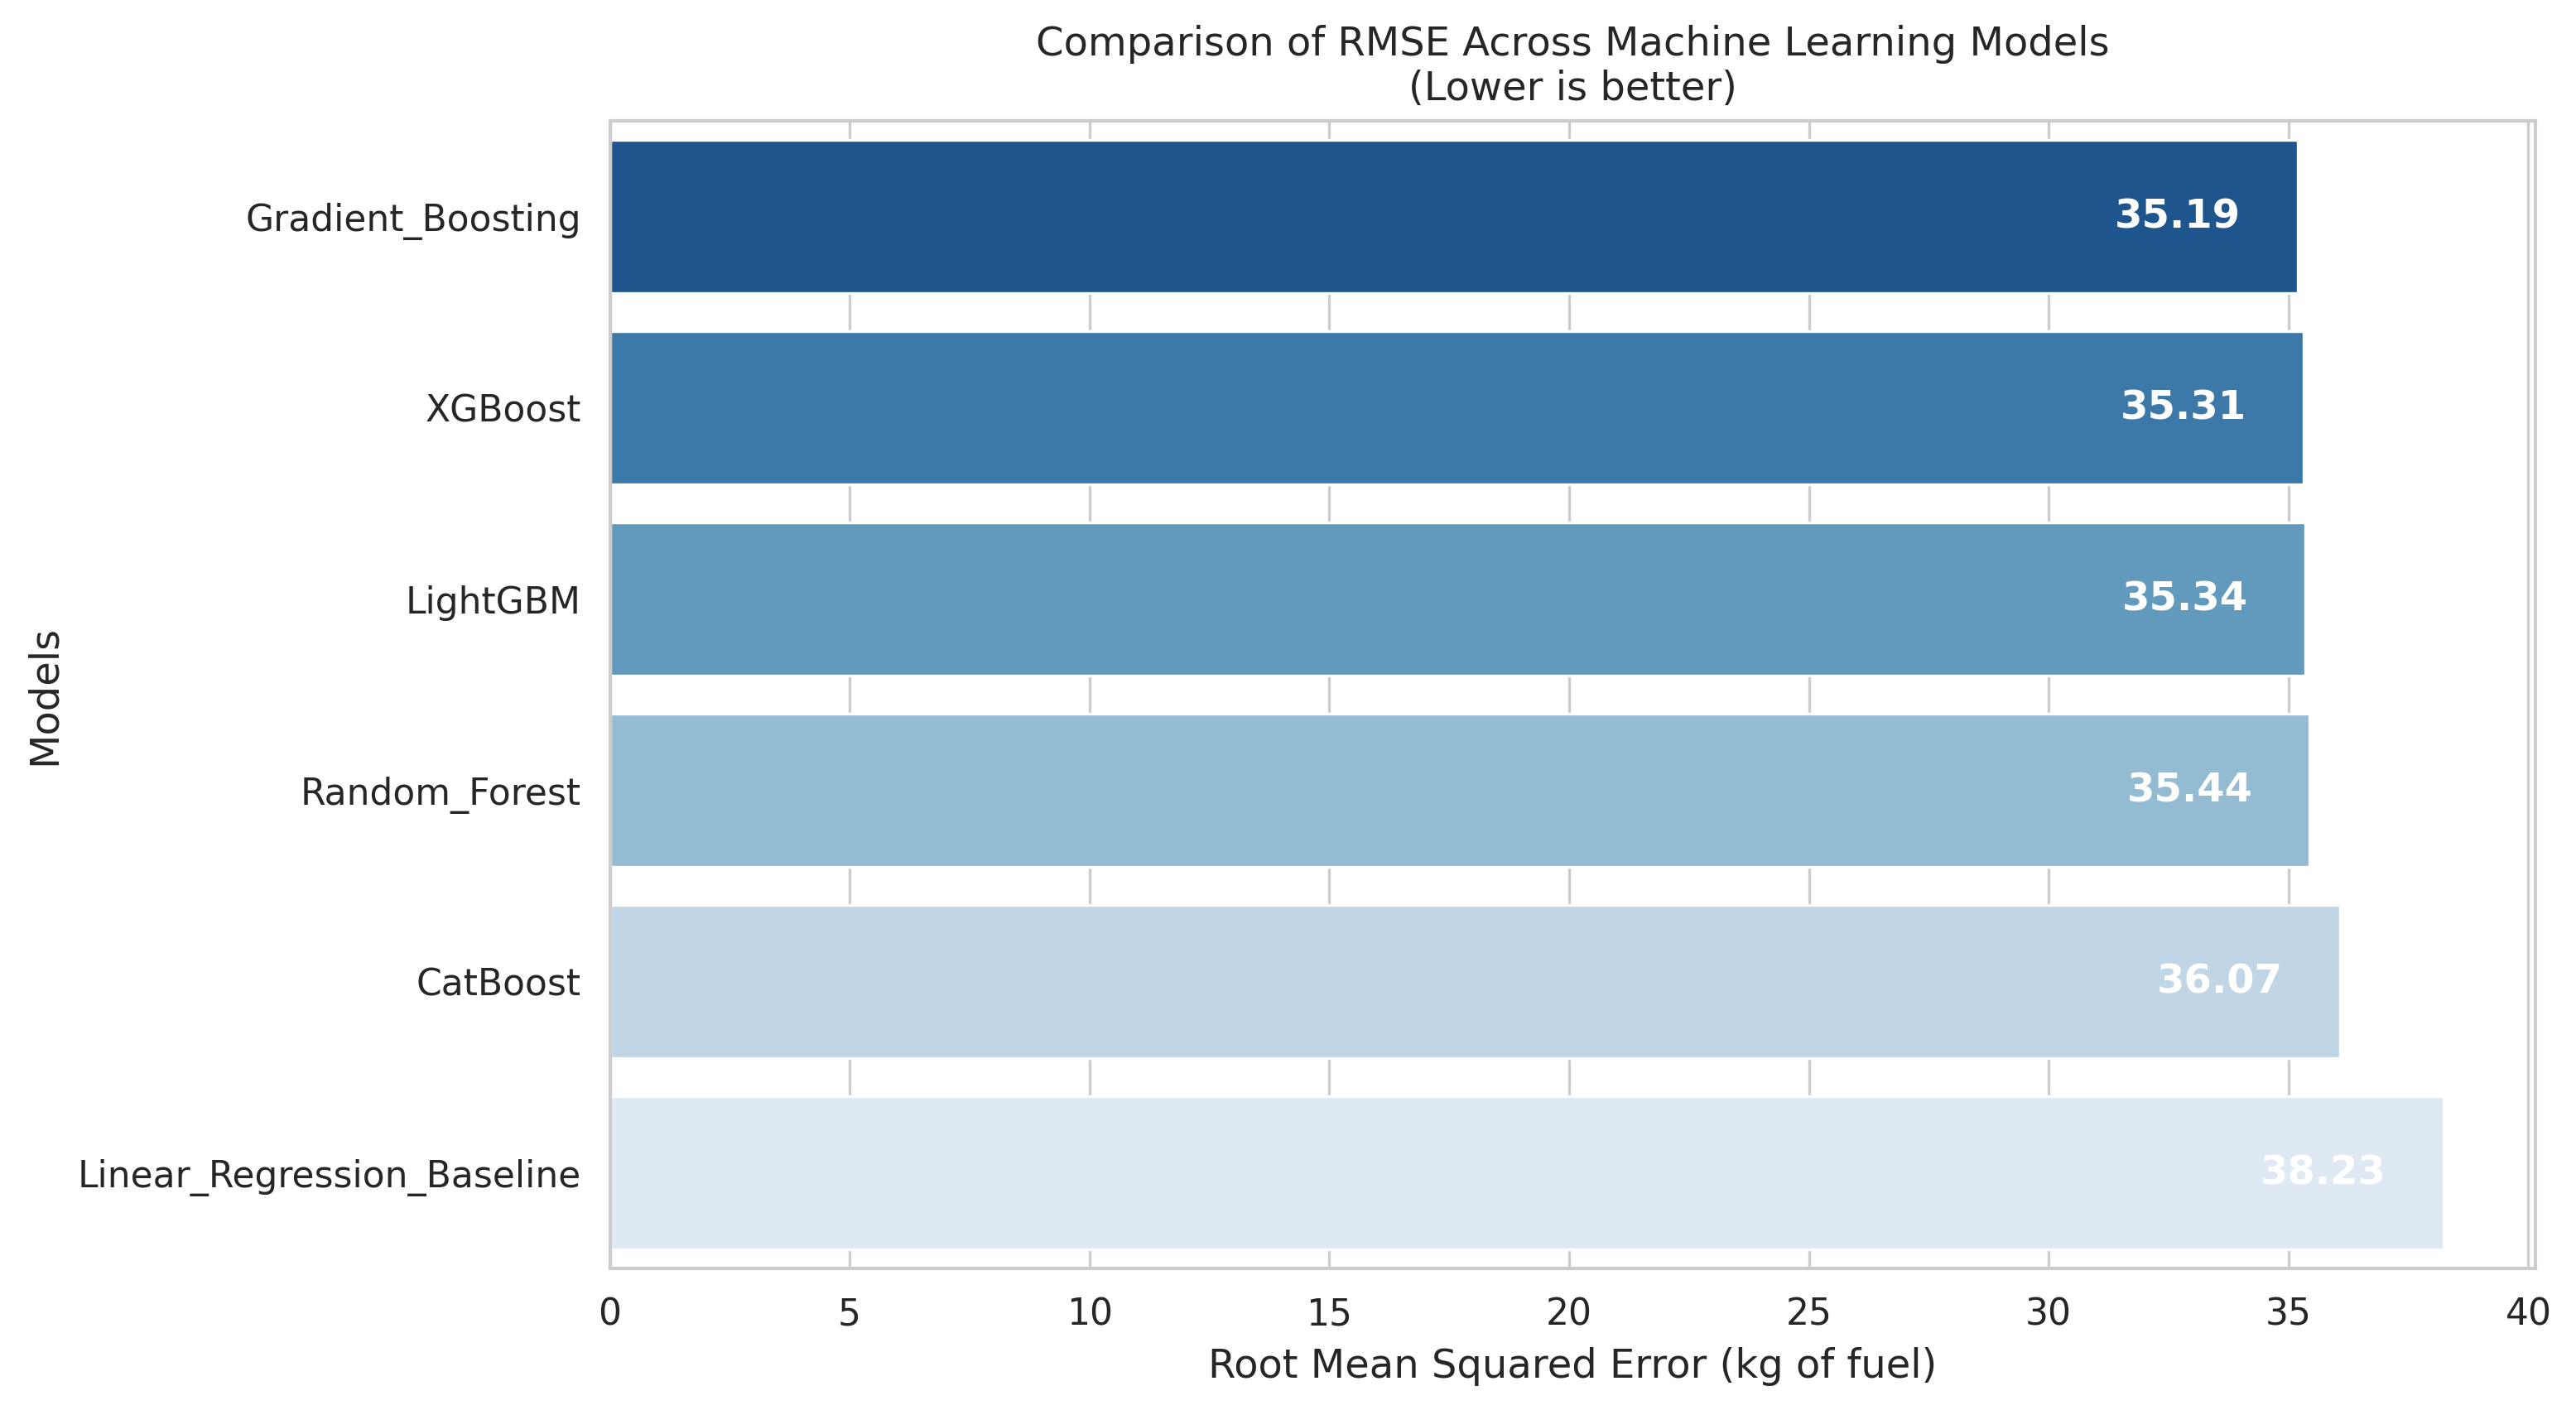
\includegraphics[width=1\linewidth]{images/comparativo_rmse.png}
    \caption{Root Mean Squared Error (RMSE) comparison across the evaluated machine learning models.}
    \label{fig:comparativo_rmse}
\end{figure}

\begin{figure}[htbp]
    \centering
    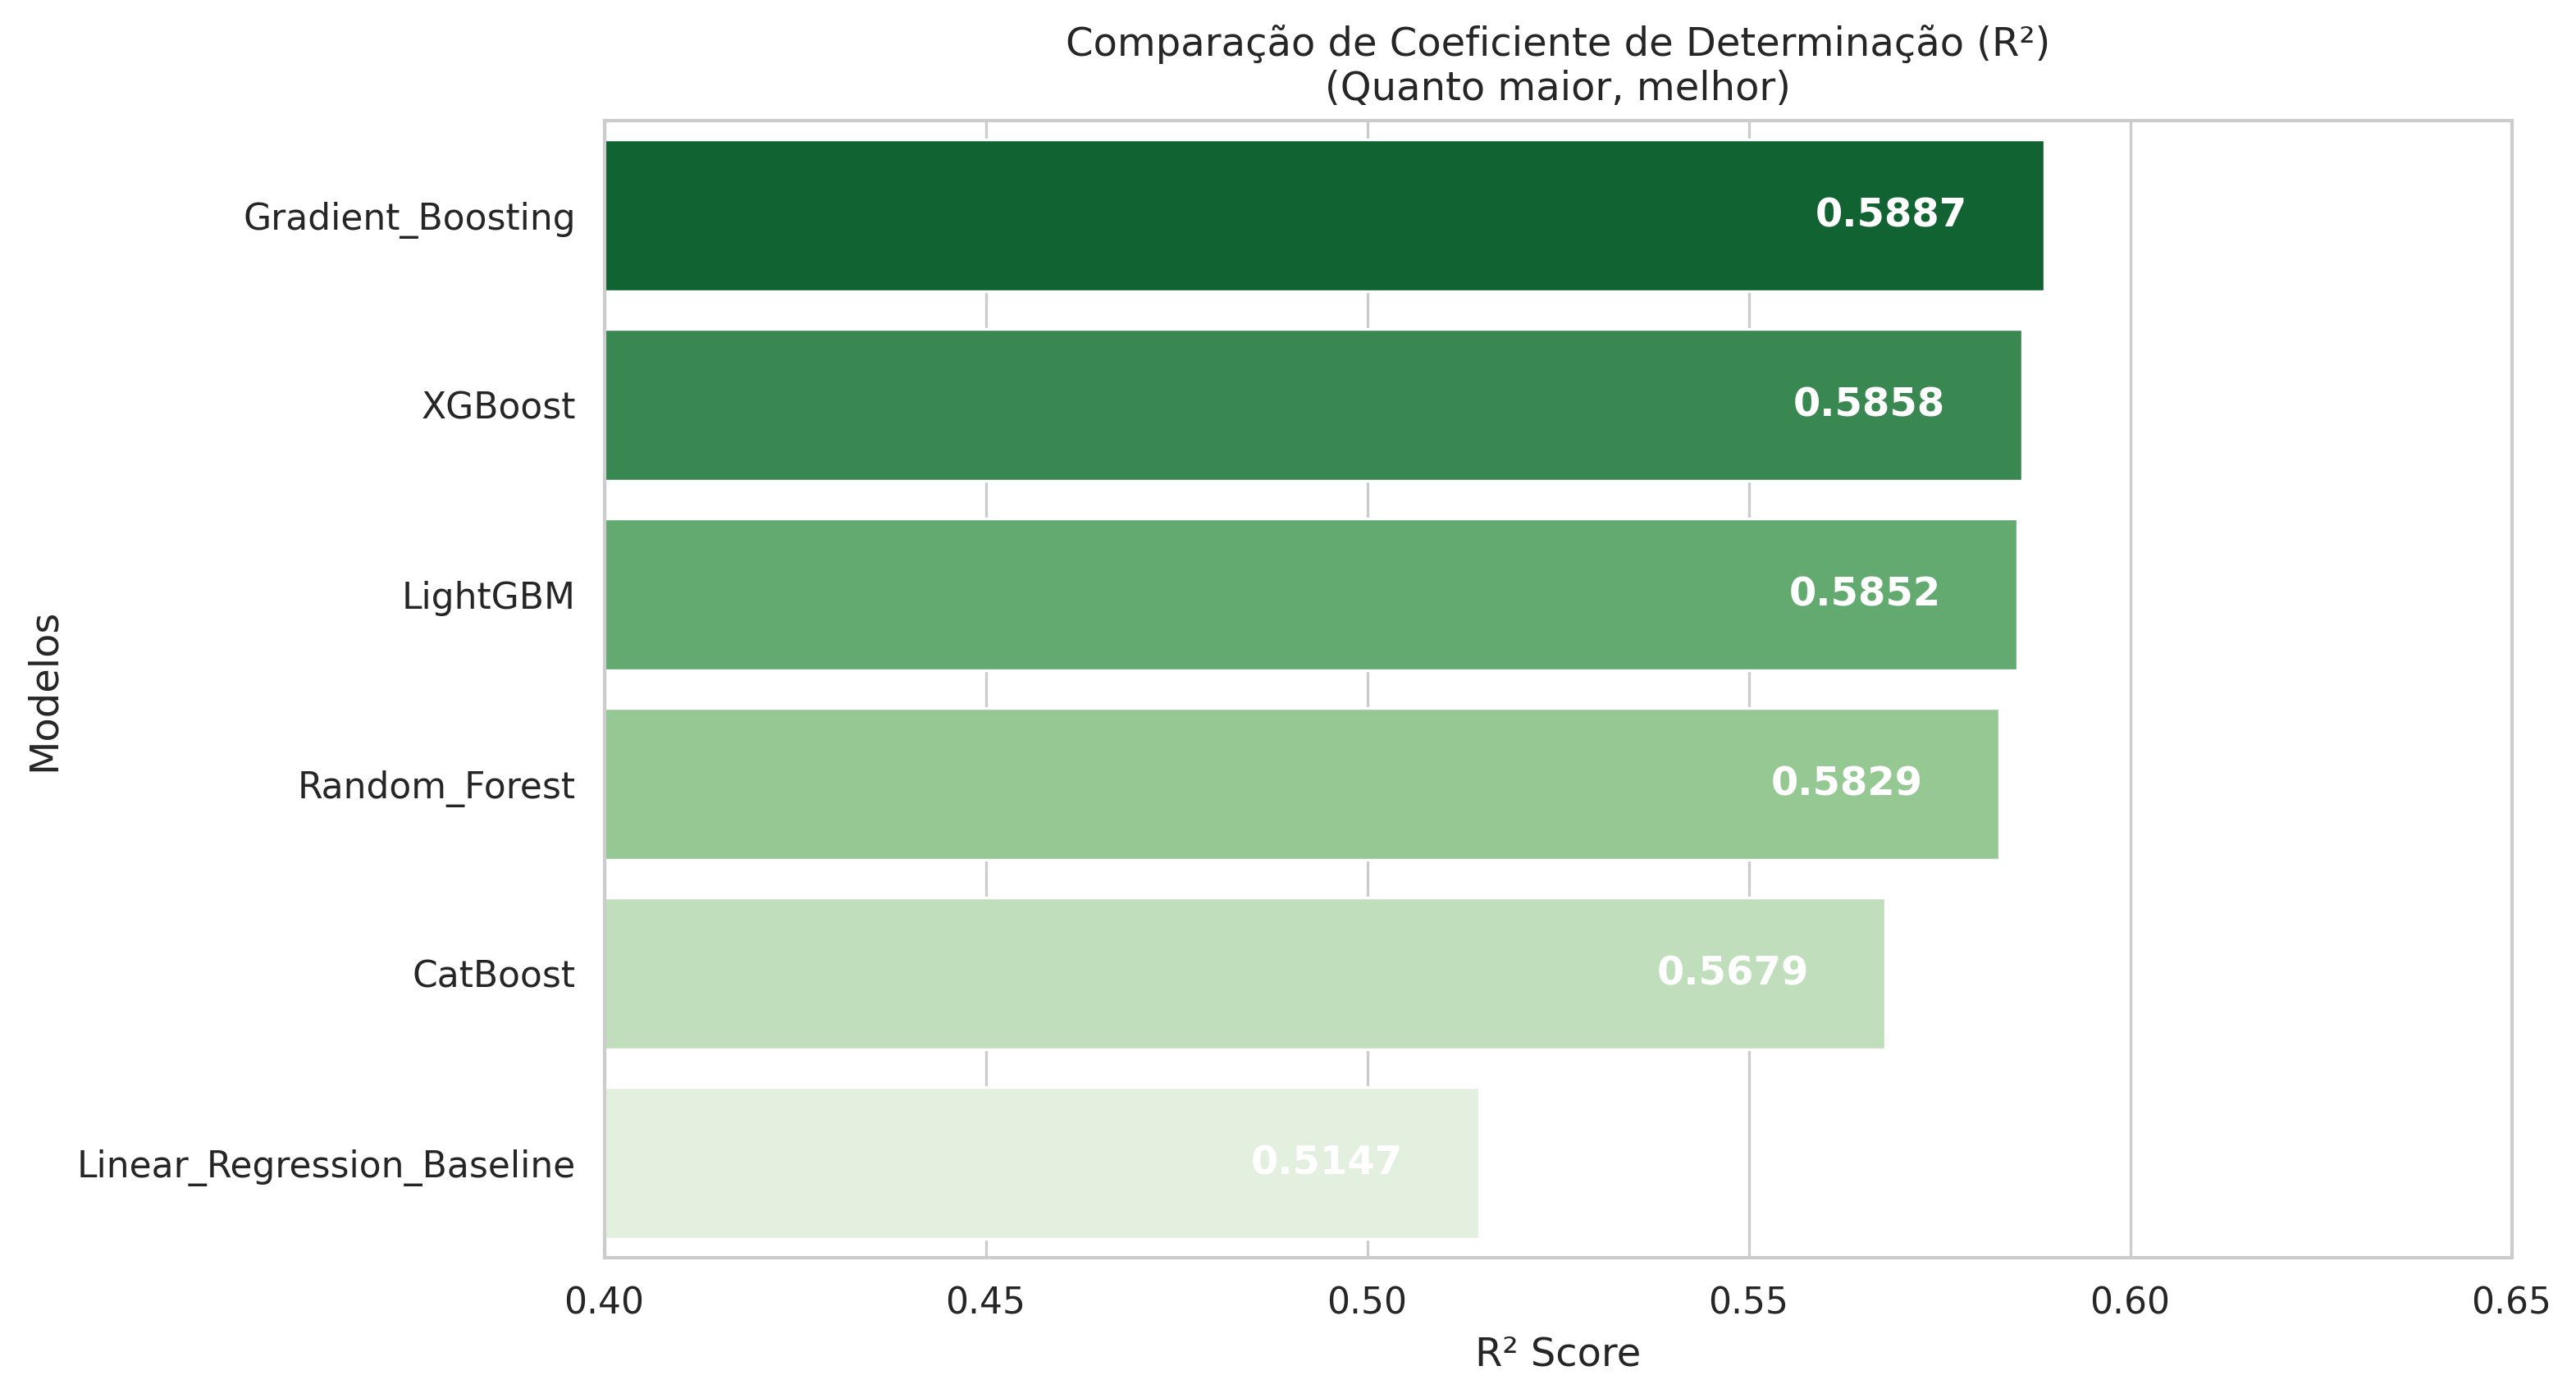
\includegraphics[width=1\linewidth]{images/comparativo_r2.png}
    \caption{Coefficient of Determination ($R^2$) comparison across the evaluated machine learning models.}
    \label{fig:comparativo_r2}
\end{figure}

As observed in Figures \ref{fig:comparativo_rmse} and \ref{fig:comparativo_r2}, all tree-based ensemble methods (Random Forest, Gradient Boosting, XGBoost, LightGBM, and CatBoost) significantly outperformed the Linear Regression baseline, which achieved an $R^2$ of 0.5147 and an RMSE of 38.23 kg. This substantial gap (an improvement of approximately 14\% in $R^2$ variance explained) underscores the highly non-linear nature of air traffic dynamics and the necessity of using advanced algorithms to capture complex interactions between arrival sectors, time of day, and congestion levels.

Among the ensemble methods, the performances were remarkably competitive. The standard Gradient Boosting Regressor (Scikit-Learn implementation) yielded the best overall results, reaching an $R^2$ of 0.5887 and an RMSE of 35.19 kg. It was closely followed by XGBoost and LightGBM. The slightly inferior performance of CatBoost in this specific setup ($R^2$ = 0.5679) can likely be attributed to the fact that we fed it a pre-encoded (One-Hot) dataset to maintain consistency across the benchmark, whereas CatBoost is specifically optimized to internally process native ordinal categorical data.

Overall, explaining nearly 59\% of the variance in additional fuel consumption ($KPI16$) is a highly promising result for an operational air traffic model. Predicting tactical fuel penalties prior to TMA entry enables controllers to anticipate bottlenecks and allows airlines to optimize their fuel policies dynamically.
